\section{System Operasi Semaphore}

	\subsection{Definisi}
	
		\begin{figure}[ht]
			\centerline{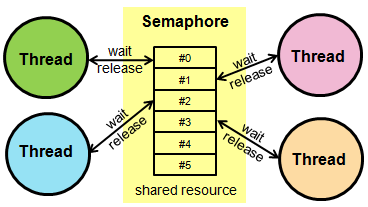
\includegraphics[width=0.5\textwidth]{figures/sema.png}}
			\caption{Semaphore}
			\label{sema}
			\end{figure}
	
		Semaphore pada system operasi merupakan sebuah variabel bertipe integer. Di kehidupan nyata, semaphore merupakan sistem sinyal yang digunakan untuk memberi sinyal atau tanda dan berkomunikasi secara visual. 
		Semafor juga merupakan struktur data dalam bahasa komputer yang digunakan untuk menyinkronkan suatu proses, yaitu untuk memecahkan masalah di mana masalahnya lebih dari satu proses atau bisa 
		seperti thread yang akan dijalankan secara bersamaan dan harus diatur urutan kerja. Semaphore dibuat oleh Edsger Dijkstra dan pertama kali digunakan dalam sistem operasi.
		Nilai semaphore diinisialisasi dengan jumlah sumber daya yang dikontrol oleh pengguna. Dalam kasus khusus di mana ada sumber daya bersama, semaphore disebut semaphore biner. 
		Semaphore adalah solusi klasik dari dining philosophers problem, meskipun itu tidak mencegah deadlock.
		Pada software, semaphore merupakan sebuah variabel bertipe data integer yang selain saat inisialisasi, yang hanya dapat diakses melalui dua operasi standar, yaitu increment dan decrement. 
		Semaphore bisa digunakan untuk menyelesaikan masalah sinkronisasi secara umum, berdasarkan jenisnya. Semaphore hanya memiliki nilai 1 atau 0, atau lebih dari sama dengan 0. 
		Konsep semaphore pertama kali diajukan idenya oleh Edsger Dijkstra pada tahun 1967. Semaphore memiliki dua jenis, yaitu, Biner semaphore dan counting semaphore. 
		Biner semaphore tidak bisa memiliki semua jenis integer tetapi hanya memiliki 2 nilai yaitu 1 atau 0, Sering juga disebut sebagai semaphore primitive. Sedangkan Counting semaphore memiliki nilai 0, 1, sampai seterusnya atau integer lainnya. 
		Banyak sistem operasi yang tidak secara langsung menggunakan semaphore jenis ini, namun lebih banyak yang memanfaatkan semaphore jenis biner semaphore. 
		Pada semaphore ini harus diketahui bahwa, ada beberapa jenis dari counting semaphore yang salah satu jenisnya adalah semafor yang tidak bisa mencapai nilai negatif dan jenis yang lain adalah semaphore yang dapat mencapai nilai negatif. 
		Solusi dari Pembuatan Counting Semaphore adalah Binary Semaphore. Pembuatan counting semaphore banyak dilakukan para programmer untuk memenuhi alat sinkronisasi yang sesuai dengannya. 
		
	\subsection{Prinsip Semaphore}
	
		\begin{enumerate}

			\item Suatu proses yang berbeda bisa berkaitan dengan memanfaatkan sinyal - sinyal.
			\item Suatu proses dapat dihentikan oleh 
			\item Semaphore bertipe data integer yang diakses oleh dua operasi atomik standar (wait dan signal).
			\item Ada dua operasi di semaphore (Down dan UP). Yang nama aslinya : P dan V.
		
		\end{enumerate}

	\subsection{Kelemahan Semaphore}
	
		\begin{enumerate}

			\item Semaphore termasuk Low Level
			\item Dikarenaka semaphore tersebar di dalam seluruh program maka kita akan kesulitan dalam pemeliharaannya.
			\item Jika kita menghapus \"wait\" akan mengakibatkan \"nonmutual exclusion\"
			\item Jika kita menghapus \"signal\" akan mengakibatkan \"deadlock\"
			\item Jika terjadi deadlock akan sulti untuk dideteksi.

		\end{enumerate}
		
	\subsection{Semantik dan Impelementasi}
		Menghitung semaphores dilengkapi dengan dua operasi, secara historis dilambangkan sebagai P dan V (lihat § Nama operasi untuk nama alternatif). Operasi V menambahkan semaphore S, dan operasi P menurunkannya.

		Nilai semaphore S adalah jumlah unit sumber daya yang saat ini tersedia. Operasi P membuang waktu atau tidur sampai sumber daya yang dilindungi oleh semaphore menjadi tersedia, pada saat itu sumber daya segera diklaim. Operasi V adalah kebalikannya: ia membuat sumber daya tersedia lagi setelah proses selesai menggunakannya. Satu properti penting dari semaphore S adalah bahwa nilainya tidak dapat diubah kecuali dengan menggunakan operasi V dan P.

		Cara sederhana untuk memahami operasi tunggu (P) dan sinyal (V) adalah:
		
		\begin{itemize}
		
			\item menunggu: Jika nilai variabel semaphore tidak negatif, turunkan dengan 1. Jika variabel semaphore sekarang negatif, proses menunggu eksekusi diblokir (yaitu, ditambahkan ke antrian semaphore) sampai nilainya lebih besar atau sama dengan 1 Jika tidak, proses terus berjalan, setelah menggunakan satu unit sumber daya.
			\item sinyal: Menambah nilai semaphore variabel dengan 1. Setelah kenaikan, jika nilai pre-increment negatif (berarti ada proses menunggu sumber daya), ia mentransfer proses yang diblokir dari antrian menunggu semaphore ke antrean siap.
			
		\end{itemize}
		
		Banyak sistem operasi menyediakan primitif semaphore yang efisien yang membuka blokir proses menunggu ketika semaphore bertambah. Ini berarti bahwa proses tidak membuang waktu untuk memeriksa nilai semaphore yang tidak perlu.Konsep penghitungan semaphore dapat diperpanjang dengan kemampuan untuk mengklaim atau mengembalikan lebih dari satu \"unit\" dari semaphore, teknik yang diterapkan di Unix. Operasi V dan P yang dimodifikasi adalah sebagai berikut, menggunakan tanda kurung siku untuk menunjukkan operasi atom, yaitu operasi yang tampak terpisah dari perspektif proses lain:

		Semaphore pada system operasi merupakan sebuah variabel bertipe integer. Di kehidupan nyata, semaphore merupakan sistem sinyal 		yang digunakan untuk memberi sinyal atau tanda dan berkomunikasi secara visual. Pada software, semaphore merupakan sebuah variabel bertipe data integer yang selain saat inisialisasi, yang hanya dapat diakses melalui dua operasi standar, yaitu increment dan decrement.
		Semaphore bisa digunakan untuk menyelesaikan masalah sinkronisasi secara umum, berdasarkan jenisnya. Semaphore hanya memiliki nilai 1 atau 0, atau lebih dari sama dengan 0. Konsep semaphore pertama kali diajukan idenya oleh Edsger Dijkstra pada tahun 1967. Semaphore memiliki dua jenis, yaitu, Biner semaphore dan counting semaphore. Biner semaphore hanya memiliki nilai 1 atau 0, Sering juga disebut sebagai semaphore primitive. Sedangkan Counting semaphore memiliki nilai 0, 1, sampai seterusnya atau integer lainnya. Banyak sistem operasi yang tidak secara langsung menggunakan semaphore jenis ini, namun lebih banyak yang memanfaatkan semaphore jenis biner semaphore

	
	\subsection{Prinsip Semaphore}
		\begin{enumerate}

			\item Suatu proses yang berbeda bisa berkaitan dengan memanfaatkan sinyal - sinyal.
			\item Suatu proses dapat dihentikan oleh 
			\item Semaphore bertipe data integer yang diakses oleh dua operasi atomik standar (wait dan signal).
			\item Ada dua operasi di semaphore (Down dan UP). Yang nama aslinya : P dan V.
			
		\end{enumerate}
		
	\subsection{Kelemahan Semaphore}

		\begin{enumerate}

			\item Semaphore termasuk Low Level.
			\item Dikarenaka semaphore tersebar di dalam seluruh program maka kita akan kesulitan dalam pemeliharaannya.
			\item Jika kita menghapus \"wait\" akan mengakibatkan \"nonmutual exclusion\".
			\item Jika kita menghapus \"signal\" akan mengakibatkan \"deadlock\".
			\item Jika terjadi deadlock akan sulti untuk dideteksi.
			
		\begin{enumerate}
		
	\cite{luu1982apparatus}
	\cite{lauesen1975large}
	\cite{hoare1974monitors}
